% Chapter X

\chapter{Existing Heat Flux Partitioning Models} % Chapter title

\label{chap:HFP_bib} % For referencing the chapter elsewhere, use \autoref{ch:name} 

%----------------------------------------------------------------------------------------

\section{Kurul \& Podowski (1990)}


In their original work published in 1990, Kurul \& Podowski \cite{kurul_1990} proposed a complete closure for the wall heat flux partitioning. They considered the applied heat flux to be divided between three mechanisms:

\begin{itemize}
\item A liquid single-phase heat flux $\phi_{c,L}$ ;
\item A boiling heat flux $\phi_{e}$ ;
\item A quenching heat flux $\phi_{q}$ induced by bubbles leaving the surface.
\end{itemize}

The total wall heat flux being :

\begin{align}
\phi_{w}=\phi_{c,L}+\phi_{e}+\phi_{q}
\end{align}

The convective heat flux is expressed as :
\begin{align}
\phi_{c,l}=A_{c,L} \rho_{L} c_{p,L}U_{L,\delta} \St_{L,\delta}\parth{T_{w}-T_{L,\delta}}
\label{eq:HFP_KP_phiCL}
\end{align}
with $\delta$ a location in the buffer layer.

Assuming bubbles are spherical and leave the surface at diameter $D_{lo}$, they write:
\begin{align}
\phi_{e}=\frac{1}{6}\pi {D_{lo}}^{3}\rho_{V}h_{LV}fN_{sit}\\
\label{eq:HFP_KP_phiE}
\end{align}

The quenching heat flux occurring over the wait time $t_{w}$ between two nucleated bubbles is computed as:  
\begin{align}
\phi_{q}=t_{w}fA_{q}\frac{2\lambda_{L}\parth{T_{w}-T_{L,\delta}}}{\sqrt{\pi \eta_{L} t_{w}}}
\label{eq:HFP_KP_phiQ}
\end{align}

This expression corresponds to the average heat flux for semi-infinite conduction over a time $t_{w}$, as expressed by Del Valle and Kenning \cite{delValle}.

They also estimate the portion of the surface affected by the bubbles as:

\begin{align}
A_{q}=\mathrm{min}\parth{1\ ;\ F_{A}\pi R_{lo}^{2} N_{sit}}=1-A_{c,L}
\label{eq:HFP_KP_AQ}
\end{align}
where $F_{A}=4$ accounts for the bubble influence area when leaving the surface.

\npar

\textbf{\underline{Needed closure relationships : }} $N_{sit}$, $f$, $t_{w}$, $D_{lo}$ 

%------------------------------------------------

\section{Basu (2000)}

In 2005, Basu \etal \cite{basu2005, basu2005a} proposed a new HFP model together with a series of experiments to further study the different needed closure relationships. This model was meant to account for finer descriptions of the multiple phenomena at stake in subcooled flow boiling. In particular, they account for bubble sliding and merging and thus distinguish bubble departure diameter $D_{d}$ (leaving the nucleation site) and lift-off diameter $D_{lo}$ (leaving the wall).

Their approach consist of separating the boiling flow in three regions (Figure \ref{fig:Basu_zones}):

\begin{itemize}
\item Pre-ONB zone, where only liquid forced convection occurs, yielding:

\begin{equation}
\phi_{w}=h_{c,L} \parth{T_{w}-T_{L}}
\label{eq:HFP_B_preONB}
\end{equation}

\item Zone between the ONB and the OSV, prior to observing a net amount of vapor with bubble lifting off the surface. The heat flux is then still totally transferred to the liquid, but the equivalent convective heat transfer coefficient is supposed enhanced by 30\% due to the presence of bubbles on the wall:

\begin{equation}
\phi_{w}=\overline{h_{c,L}} \parth{T_{w}-T_{L}}\approx 1.3 h_{c,L}\parth{T_{w}-T_{L}}
\label{eq:HFP_B_postONB}
\end{equation}

Basu \etal define the ONB as:

\begin{align}
&T_{w, ONB}= T_{sat} + \frac{4 \sigma T_{sat}}{D_{c}\rho_{V} h_{LV}}\\
%
&D_{c}= \sqrt{\frac{8 \sigma T_{sat} \lambda_{L}}{\rho_{V} h_{LV} \phi_{w}}}\parth{ 1- \exp{ - \theta^{3} - 0.5 \theta}  }
\label{eq:HFP_B_ONB}
\end{align}

\item Post-OSV zone, where bubbles now leave the surface towards the bulk flow. This is where the other parts of the HFP appear \ie the boiling and quenching fluxes. The beginning of OSV is defined by Basu \etal as:

\begin{equation}
T_{L,OSV}=T_{sat}-0.7\exp{-0.065 \frac{D_{d}h_{c,L}}{\lambda_{L}}}\frac{\phi_{w}}{h_{c,L}}
\end{equation}

\end{itemize}


\begin{figure}[h]
\centering
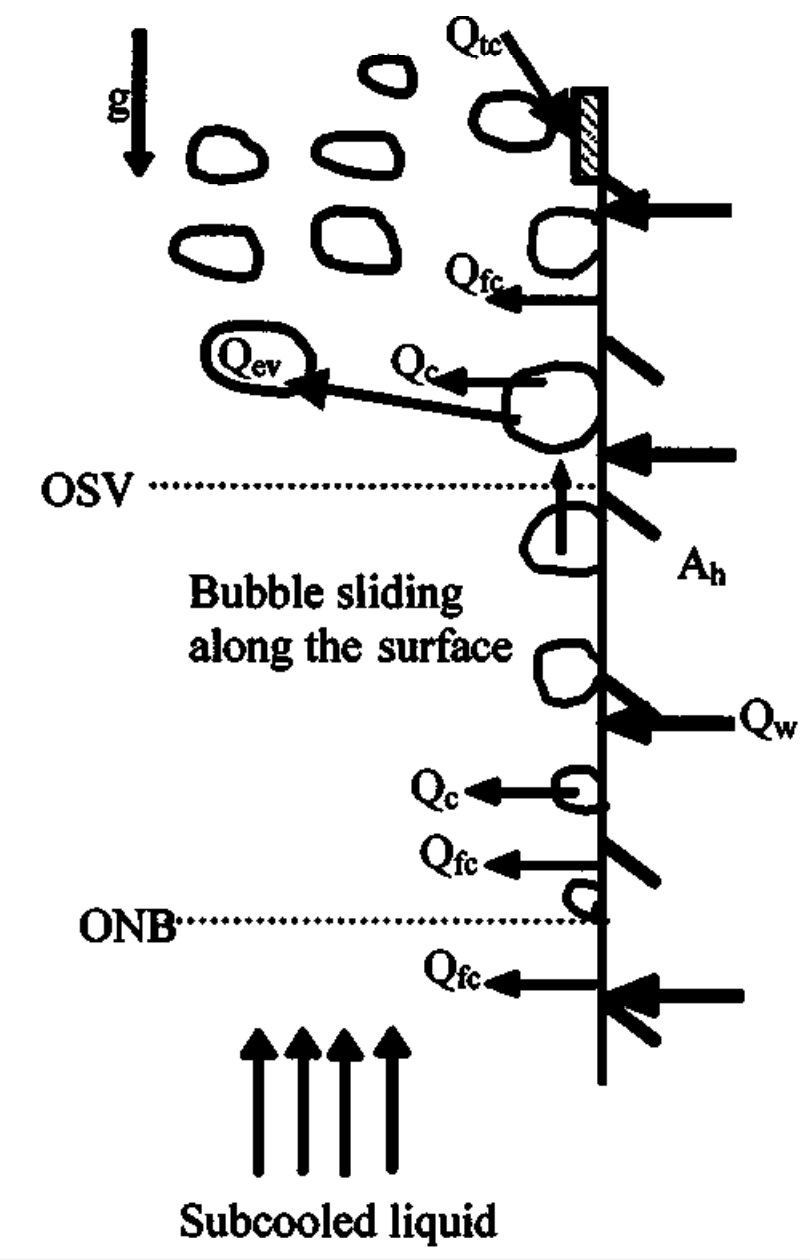
\includegraphics[width=0.5\linewidth]{img/HFP/Basu/zones.PNG}
\caption{Sketch of the heat transfers zones considered by Basu \etal. (Adapted from \cite{basu2005})}
\label{fig:Basu_zones}
\end{figure}
	

The hypothesis of Basu \etal is that the heat flux is first transferred to the superheated liquid close to the wall (by convection and transient quenching), part of which contributing to the evaporation through the liquid-vapor interface. The remaining heat is transferred to the bulk liquid ($\phi_{L}$) either from the superheated liquid layer or bubble condensation. The whole heat transfer mechanism can thus be written as:

\begin{equation}
\phi_{w} = \phi_{c,L}+\phi_{q} = \phi_{e} + \phi_{L}
\label{eq:HFP_B_tot}
\end{equation}

In order to estimate the quenching heat flux associated to bubble sliding and lift-off, Basu \etal consider two cases: 

\begin{itemize}
\item[1)] Bubble sliding from departure ($D=D_{d}$) to lift-off ($D=D_{lo}$) ;
\item[2)] Bubble coalescence with neighboring sites before departure.
\end{itemize} 

Those two cases are distinguished using the average distance between nucleation sites $s$, which they suppose equal to $1/\sqrt{N_{sit}}$.

\subsection{Case 1 : Bubble sliding, $D_{d}<s$}

In this situation, the bubble will grow up to its departure diameter $D_{d}$ and slide over a length $l_{sl,0}$ before lifting-off. If $l_{sl,0}<s$, the bubble will slide up to its lift-off diameter $D_{l}$ and leave the wall withouth colliding with other bubbles. On the contrary, if $l_{sl,0}\geq s$ the sliding bubble will merge with bubbles growing on their nucleation site, inducing a sudden growth of the bubble diameter that can exceed $D_{lo}$ and thus lift-off after sliding over a reduced length $l_{sl}<l_{sl,0}$. Those assumptions are summarized on Figure \ref{fig:Basu_sliding}.

\begin{figure}[h]
\centering
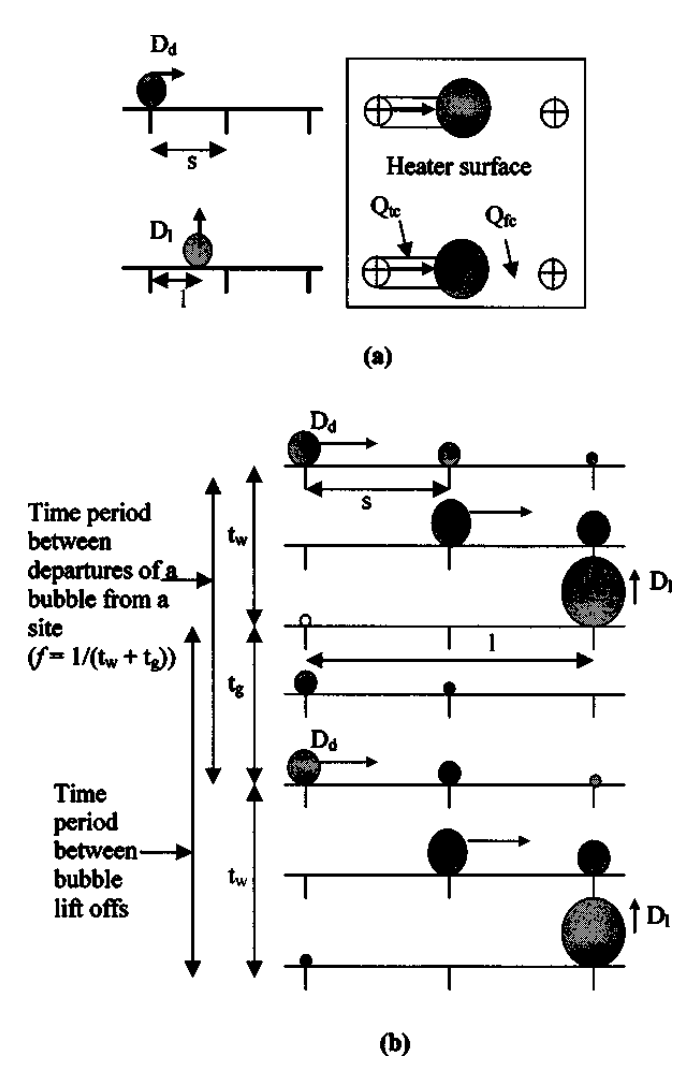
\includegraphics[width=0.5\linewidth]{img/HFP/Basu/slide.PNG}
\caption{Sliding bubble behavior considered by Basu \etal. (Adapted from \cite{basu2005})}
\label{fig:Basu_sliding}
\end{figure}
	

If bubble coalescence occurs, the number of bubbles lifting-off the surface is lower than the actual number of nucleating sites. Basu \etal thus define a reduction factor:

\begin{align}
R_{f}&=
\begin{dcases}
\dfrac{s}{l_{sl}} = \dfrac{1}{l\sqrt{N_{sit}}} & \text{if } l_{sl,0} \geq s \\
1 & \text{if } l_{sl,0}<s
\end{dcases}
\label{eq:HFP_B_Rf}
\end{align}  


Regarding bubble sizes, they suppose that bubbles coalesced by a sliding bubble while growing have a diameter $D_{d}$ \ie they were close to departure (in reality, the coalesced bubble would have a diameter $D<D_{d}$). This results in a bubble of diameter $D=\parth{D_{sl}^{3} + D_{d}^{3}}^{1/3}$ which will lift-off id $D>D_{lo}$. Consequently, a sliding bubble can merge with numerous bubbles before lifting off. Noting $N_{merg}$ the number of coalesced bubble and $D_{N}$ the resulting bubble diameter, the sliding distance is:

\begin{equation}
l_{sl}=N_{merg}s + l_{D_{N}\rightarrow D_{lo}}
\end{equation}
where $l_{D_{N}\rightarrow D_{lo}}$ is the remaining distance to slide if $D_{N}<D_{lo}$, being $0$ if $D_{N}>D_{lo}$.

The surface swiped by the sliding bubble is then expressed as $A_{sl} = C\overline{D}l_{sl}$ with $\overline{D}$ the average bubble diameter during sliding and $C$ the ration between the bubble diameter and its foot, expressed correlating measurements from Maity \cite{maity2000} as :

\begin{equation}
C=1-\exp{2-\theta ^{0.6}}
\end{equation}

After observing in their experiments that $D_{d}\approx 0.5D_{lo}$, Basu \etal choose:

\begin{equation}
\overline{D}=\frac{D_{lo}+D_{d}}{2}\approx 0.75D_{lo}
\end{equation}

Noting $t^{*}=\parth{\dfrac{\lambda_{L}}{h_{c,L}}}^{2} \dfrac{1}{\pi \eta_{L}}$ the time at which transient conduction heat transfer becomes equal to forced liquid convection, the quenching heat flux is expressed as:

\begin{equation}
\phi_{q} = \frac{1}{t_{w}+t_{g}} \int_{0}^{T}\frac{\lambda_{L}}{\sqrt{\pi \eta_{L}t}}\parth{T_{w}-T_{L}}A_{sl}R_{f}N_{sit}dt
\end{equation}
where $T=t^{*}$ if $t^{*}<t_{w}+t_{g}$ (forced convection dominates at some point during a nucleation cycle) or $T=t_{w}+t_{g}$ if $t^{*}\geq t_{w}+t_{g}$ (transient conduction dominates over the whole nucleation cycle).

\npar
The liquid convective heat transfer is then:

\begin{equation}
\phi_{c,L} = \overline{h_{c,L}}\parth{T_{w}-T_{L}}A_{c,L} + \overline{h_{c,L}}\parth{T_{w}-T_{L}}A_{sl}R_{f}N_{sit}\parth{1-\mathrm{min}\parth{1\ ;\ \frac{t^{*}}{t_{w}+t_{g}}}}
\label{eq:HFP_B_phiCL}
\end{equation}
with $A_{c,L} = 1 - A_{sl}R_{f}N_{sit}$.

And the boiling heat flux:

\begin{equation}
\phi_{e} = \rho_{V}h_{LV}\frac{\pi}{6}D_{lo}^{3}R_{f}N_{sit}\frac{1}{t_{w}+t_{g}}
\label{eq:HFP_B_phiE}
\end{equation}


\subsection{Case 2 : Bubble coalesence without sliding, $D_{d}\geq s$}

Under higher wall superheats, the subsequent rise in the nucleation site density $N_{sit}$ can lead to boiling regimes where bubbles coalesce with each other at early stages of their lifetime \ie while still attached to their nucleation site. This situation is accounted for by Basu \etal in the case when $D_{d} \geq s$ by considering immediate lift-off of coalesced bubble at radius $D > D_{lo}$. In this case, the total number of bubbles leaving the surface is lower than $N_{sit}$ and is thus reduced using:

\begin{equation}
R_{f} = \frac{s^{3}}{D_{lo}^{3}}
\end{equation}

Under this massive coalescing regime, the entire surface will experience quenching due to bubble lift-off all over the heater. Depending on the values of $t^{*}$, we have:

\begin{align}
\phi_{q} &= 
\begin{dcases} \dfrac{1}{t_{w}+t_{g}} \int_{0}^{t^{*}}\dfrac{\lambda_{L}}{\sqrt{\pi \eta_{L}t}}\parth{T_{w}-T_{L}}dt & \text{if } t^{*}<t_{w} \\
%
\dfrac{1}{t_{w}+t_{g}} \crocht{ \int_{0}^{t_{w}}\dfrac{\lambda_{L}}{\sqrt{\pi \eta_{L}t}}\parth{T_{w}-T_{L}}dt + \int_{0}^{T}\dfrac{\lambda_{L}}{\sqrt{\pi \eta_{L}t}}\parth{T_{w}-T_{L}}\crocht{1-S_{b}N_{sit}}dt} & \text{if } t^{*}\geq t_{w} 
\end{dcases}
\end{align}

\begin{align}
\phi_{c,L} &= 
\begin{dcases} \overline{h_{c,L}}\parth{T_{w}-T_{L}}\frac{t_{w}-t^{*}}{t_{w}+t_{g}} + \overline{h_{c,L}}\parth{T_{w}-T_{L}}\crocht{1-A_{b}N_{sit}}\frac{t_{g}}{t_{w}+t_{g}} & \text{if } t^{*}<t_{w} \\
%
\overline{h_{c,L}}\parth{T_{w}-T_{L}}\crocht{1-A_{b}N_{sit}}\frac{t_{w}+t_{g}-t^{*}}{t_{w}+t_{g}} & \text{if } t^{*}\geq t_{w} 
\end{dcases}
\end{align}
with $A_{b} = \dfrac{\pi \parth{Cs}2}{4}$.

And the boiling heat flux still expressed as Eq. \ref{eq:HFP_B_phiE}.

\npar


\textbf{\underline{Needed closure relationships : }} $N_{sit}$, $t_{w}$, $t_{g}$, $D_{d}$, $D_{lo}$, $l_{sl,0}$, $h_{c,L}$. 


%----------------------------------------------------------------------------------------

\section{Gilman (2017)}

A more recent HFP model dedicated to CFD simulations has been proposed by Gilman \& Baglietto in 2017 \cite{gilman2017}. Among the different advances proposed in their work, we can mention :

\begin{itemize}
\item A probabilistic law to account for static interaction between nucleation sites ;
\item A force-balance approach to compute the bubble departure and lift-off diameters ;
\item A generic law for the enhanced forced convection coefficient accounting for bubble presence ; 
\item The presence of a modified quenching term accounting for local wall superheat beneath a bubble dry spot.
\end{itemize}

The total heat flux is partitioned between the liquid forced convection $\phi_{c,L}$, the solid quenching $\phi_{q,s}$, the quenching due to bubble sliding $\phi_{q,sl}$ and the evaporation flux $\phi_{e}$. Yielding:

\begin{equation}
\phi_{w} = \phi_{c,L} + \phi_{q,s} + \phi_{q,sl} + \phi_{e}
\end{equation} 

The convective term is computed in a way similar to Basu \etal \cite{basu2005} in Eq. \ref{eq:HFP_B_phiCL}:

\begin{align}
\phi_{c,L} =& \phi_{c1,L} + \phi_{c2,L}\\
% 
=&h_{c,L}\parth{1-A_{sl}N_{sit,a}^{*}}\parth{T_{w}-T_{L}} + \overline{h_{c,L}}A_{sl}N_{sit,a}^{*}\parth{1 - \frac{t^{*}}{t_{w}+t_{g}}}\parth{T_{w}-T_{L}}
\end{align}
where $N_{sit,a}^{*}$ is the active nucleation site density that will generate sliding bubbles, that can differ from the empirical value of available sites $N_{sit}$ usually computed by a correlation. 

The active nucleation site density is actually smaller than $N_{sit}$ since Gilman considers an static interaction between the available sites \ie the fact that a bubble laying on a site may be blocking nucleation from sites laying beneath its foot. Following a Complete Spatial Randomness (CSR) approach, they express the probability to find a site under a growing bubble of radius $R_{d}$ as:

\begin{equation}
\mathcal{P} = 1-e^{-N_{b}\pi R_{d}^{2}}
\label{eq:HFP_G_Pinter}
\end{equation} 
where $N_{b} = \dfrac{t_{g}}{t_{w}+t_{g}}N_{sit}$ is the density of bubbles covering the heater.

The number of active sites is then computed as:

\begin{align}
N_{sit,a} &= \parth{1-\mathcal{P}}N_{sit}\\
%
&= \exp{-\dfrac{t_{g}}{t_{w}+t_{g}}N_{sit}\pi R_{d}^{2}} N_{sit}
\label{eq:HFP_G_Nsita}
\end{align}

This value is then reduced by Gilman to obtain $N_{sit,a}^{*}$ using a reduction factor representing sliding bubble coalesence (similar to Basu in Eq. \ref{eq:HFP_B_Rf}):

\begin{equation}
N_{sit,a}^{*}=R_{f}N_{sit,a} = \frac{s}{l_{sl,0}+s} N_{sit,a}
\end{equation}


The sliding quenching term is also computed in a similar way to Basu as:

\begin{align}
\phi_{q,sl}&=\frac{2\lambda_{L}\parth{T_{w}-T_{L}}}{\sqrt{\pi \eta_{L}t^{*}}}A_{sl}N_{sit,a}^{*} \\
%
A_{sl} &= \overline{D}l_{sl} = \frac{D_{d}+D_{lo}}{2}\parth{N_{merg}s+l_{D_{N}\rightarrow D_{lo}}}
\end{align}

Regarding the boiling heat flux, Gilman splits it in two contributions respectively associated with the inception of nucleation and liquid microlayer evaporation :

\begin{align}
\phi_{e} =& \phi_{e,init} + \phi_{e,ML} \\
%
=& \frac{4}{3}\pi R_{d}^{3}\rho_{V} h_{LV} \frac{1}{t_{w}+t_{g}}N_{sit,a} + V_{ML} \rho_{L}h_{LV} \frac{1}{t_{w}+t_{g}}N_{sit,a}\\
%\
\text{with } V_{ML} =& \frac{2}{3}\pi \parth{\frac{R_{d}}{2}}^{3}\delta_{max}
\end{align}
where $\delta_{max}=2\ \mu\text{m}$ based on experiments from Gerardi \cite{gerardi}.


Finally, the solid quenching term is written as:

\begin{align}
& \phi_{q,s} = \rho_{w} c_{p,w} V_{q} \delta T_{q} \frac{1}{t_{g}+t_{w}} N_{sit,a}\\
%
& V_{q} = \frac{2}{3} \pi r_{w}^{2}
\end{align}
with $\Delta T_{q}=2\ K$ as suggested by Gerardi \etal \cite{gerardi_etal}.

\npar

\textbf{\underline{Needed closure relationships : }} $N_{sit}$, $t_{w}$, $t_{g}$, $D_{d}$, $D_{lo}$, $l_{sl,0}$, $h_{c,L}$, $\overline{h_{c,L}}$. 



\section{Zhou (2020)}

The last HFP model we will look through in this Chapter was proposed by Zhou \etal \cite{zhou}. It is one of the most recent available in the literature and was built along with associated experiments for validation. In particular they compute separate heat flux contributions for static ($st$) or sliding bubbles ($sl$), yielding a total heat flux:

\begin{equation}
\phi_{w} = \phi_{c,L} + \parth{\phi_{e,st}+ \phi_{e,st}} + \parth{\phi_{e,sl}+\phi_{q,sl}}
\end{equation}

An interesting aspect of Zhou \etal work is the presence of a condensation term in the evaporation heat fluxes, written as:

\begin{align}
\phi_{e,st} =& \rho_{V}h_{LV}\frac{4}{3}\pi R_{d}^{3} N_{sit,a} f  + h_{cond}\parth{T_{sat}-T_{L}}A_{cond} N_{sit,a} f \parth{t_{g}-t_{s}} \\
%
\phi_{e,sl} =& \frac{\pi}{6}\rho_{V}h_{LV}\parth{D_{lo}^{3}-D_{d}^{3}}fN_{sit}^{*} + h_{cond} \parth{T_{sat}-T_{L}}A_{cond}N_{sit}^{*}t_{sl}f\\
%
A_{cond} =& \pi D_{d} \mathrm{max}\parth{R_{d}\parth{1+\cos{\theta}}-y_{sat}\ ;\ 0}
\end{align}
where $y_{sat}$ is the wall distance where the liquid is at saturation temperature, $t_{s}$ the moment when $D_{b}=y_{sat}$ and $N_{sit}^{*}$ the number of sliding bubbles.

The condensation heat transfer coefficient is computed using the correlation from Ranz \& Marshall:

\begin{equation}
h_{cond} = \frac{\lambda_{L}}{D_{d}}\parth{2+0.6\Re_{b}^{0.5}}\Pr_{L}^{0.3}
\end{equation}

Following similar approaches to HFP models from Basu or Gilman, the quenching heat flux for static bubbles is expressed as:

\begin{align}
\phi_{q,st}&=
\begin{dcases}
t_{w}f\frac{2\lambda_{L}\parth{T_{w}-T_{L}}}{\sqrt{\pi \eta_{L}t_{w}}}A_{b}N_{sit} & \text{if } t^{*} \geq t_{w}\\
%
t^{*}f\frac{2\lambda_{L}\parth{T_{w}-T_{L}}}{\sqrt{\pi \eta_{L}t^{*}}}A_{b}N_{sit} + h_{c,L}\parth{T_{w}-T_{L}}A_{b}N_{sit}^{*}f\parth{t_{w}-t^{*}} & \text{if } t^{*}<t_{w}
\end{dcases}
\end{align}
with $A_{b}= \underbrace{K_{b}}_{=2} \pi R_{d}^{2}$.

And for the sliding bubbles:

\begin{align}
\phi_{q,sl}&=
\begin{dcases}
\frac{2\lambda_{L}\parth{T_{w}-T_{L}}}{\sqrt{\pi \eta_{L}\parth{t_{g}+t_{w}}}}A_{sl}N_{sit}^{*} & \text{if } t^{*} \geq t_{g}+t_{w}\\
%
t^{*}f \frac{2\lambda_{L}\parth{T_{w}-T_{L}}}{\sqrt{\pi \eta_{L}t^{*}}}A_{b}N_{sit}^{*} + h_{c,L}\parth{T_{w}-T_{L}}A_{sl}N_{sit}^{*}f\parth{t_{g}+t_{w}-t^{*}} & \text{if } t^{*}<t_{w}
\end{dcases}
\end{align}
with $A_{sl}=\underbrace{K_{sl}}_{=2}\dfrac{D_{d}+D_{lo}}{2}l_{sl}$ and $l_{sl}=\mathrm{min}\parth{l_{sl,0}\ ;\ \dfrac{1}{\sqrt{t_{g}fN_{sit}}} }$.

Finally, the forced liquid convective heat flux is computed:

\begin{equation}
\phi_{c,L} = h_{c,L}\parth{1-A_{b}N_{sit}-A_{sl}N_{sit}^{*}}\parth{T_{w}-T_{L}}
\end{equation}

\npar

\textbf{\underline{Needed closure relationships : }} $N_{sit}$, $t_{w}$, $t_{g}$, $D_{d}$, $D_{lo}$, $l_{sl,0}$, $h_{c,L}$. 


\section{Closure Laws for Remaining Parameters}

In each of the 4 presented HFP models, there is a number of parameters that still need to be computed in order for the model to be fully expressed. Those parameters are often the nucleation site density, bubble diameters, etc. To do so, closure relationships are used and differ from one model to another. Here we want to sum up the different choices of the authors to point the variety of possibilities that exist.

\subsection{Nucleation Site Density : $N_{sit}$}

The value of the nucleation site density is a very sensitive parameter that controls the intensity of the boiling heat transfer. Unfortunately, its value can vary over a very large range of value depending on the operating conditions and heater material and is thus expressed using experimental correlations.

\npar
In their work, Kurul \& Podowski used the law of Lemmert and Chawla \cite{lemmert}:

\begin{align}
N_{sit}=\crocht{210\parth{T_{w}-T_{sat}}}^{1.8}
\end{align}


\npar
Later, Basu \cite{basu} correlated her own experimental results to obtain:

\begin{align}
N_{sit}=&
\begin{dcases}
0.34\crocht{1-\cos{\theta}} {\Delta T_{w}}^{2} & \text{if } \Delta T_{w,ONB}<\Delta T_{w} < 15\ K\\
3.4\times 10^{-5}\crocht{1-\cos{\theta}} {\Delta T_{w}}^{5.3} & \text{if } \Delta T_{w} > 15\ K
\end{dcases}
\end{align}

\npar

\npar
Finally, Zhou \etal followed a approach similar to Basu \etal by correlating their own experimental data:

\begin{align}
N_{sit} =& N_{0}\parth{1-\cos{\theta}}\crocht{\exp{\mathrm{f}\parth{P} \Delta T_{w} } -1 }
\mathrm{f}\parth{P} = 0.218~\ln{\dfrac{P}{P_{0}}}+0.1907
\end{align}
with $N_{0}=55~395.26\ \mathrm{m}^{-2}$ and $P_{0}=1.01\ \mathrm{bar}$.



\subsection{Bubble Departure Frequency $f$, Growth Time $t_{g}$ and Wait Time $t_{w}$}


Historically, Kurul \& Podowski modeled the BDF according to Cole \cite{cole} which derived an expression using photographic observations of bubble nucleation, further verified by Ceumern \& Lindenstjerna for pool boiling of water at pressures up to 8 bar. :

\begin{align}
f = \sqrt{\frac{4}{3} \frac{g \parth{\rho_{L}-\rho_{V}}}{\rho_{L}D_{d}} }
\label{eq:f_Cole}
\end{align}

Then, assuming that the growth time of the bubble before departure is small compared to the wait time before a new bubble nucleates ($t_{g,d} \ll t_{w}$) gives :

\begin{align}
t_{w} \approx \frac{1}{f}
\end{align}


Although the assumption of a negligible growth time is true in different cases, notably when bubble departure diameter is small \ie they leave their nucleation site nearly instantly, this is not generally true and the value of the ratio $\dfrac{t_{g,d}}{t_{w}}$ can vary by decades depending on the thermal-hydraulics conditions.

Thus, later models considered separate modeling of the growth and wait time in order to compute the BDF as :

\begin{align}
f = \frac{1}{t_{g,d} + t_{w} }
\label{eq:frequency}
\end{align}


In this scope, Basu \etal \cite{basu} correlated their own exprimental results to obtain :

\begin{align}
t_{g} =& \frac{D_{d}^{2} }{45~e^{-0.02~\Ja_{L}} \eta_{L} \Ja_{w}} \label{eq:tg_Basu}
 \\
t_{w} =&  139.1\ {\Delta T_{w}}^{-4.1}
\label{eq:tw_Basu}
\end{align}


Gilman \& Baglietto \cite{gilman} chose use the growth law of Zuber \cite{zuber1961} and the total BDF of Cole (Eq. \ref{eq:f_Cole}) to close the relation \ref{eq:frequency}.

\begin{align}
t_{g,d} = \frac{\pi {R_{d}}^{2}}{4b^{2} \Ja_{w} \eta{L}},\ \ b=1.56
\end{align}